\documentclass[tikz,border=2mm]{standalone}
\usepackage[margin=1in]{geometry}

% math + tikz
\usepackage{amsmath}
\usepackage{tikz}
\usetikzlibrary{decorations.pathreplacing,decorations.pathmorphing}

% your macros
\providecommand{\ket}[1]{\left|#1\right\rangle}
\providecommand{\phaseH}[1]{e^{-i{\gamma}_{#1} \hat{H}_P}}
\providecommand{\phaseM}[1]{e^{-i{\beta}_{#1} \hat{H}_M}}

\begin{document}
\centering

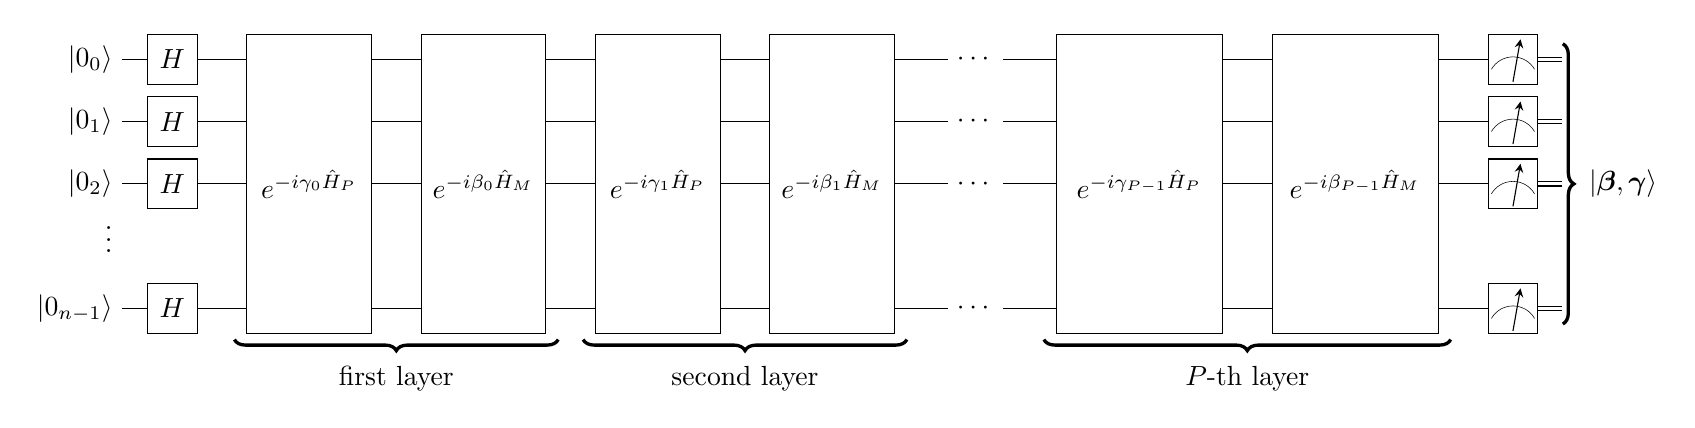
\begin{tikzpicture}[scale=1.500000,x=1pt,y=1pt]
\filldraw[color=white] (0.000000, -7.500000) rectangle (347.000000, 67.500000);
% Drawing wires
% Line 7: a0 W \ket{0_0}
\draw[color=black] (0.000000,60.000000) -- (335.000000,60.000000);
\draw[color=black] (335.000000,59.500000) -- (347.000000,59.500000);
\draw[color=black] (335.000000,60.500000) -- (347.000000,60.500000);
\draw[color=black] (0.000000,60.000000) node[left] {$\ket{0_0}$};
% Line 8: a1 W \ket{0_1}
\draw[color=black] (0.000000,45.000000) -- (335.000000,45.000000);
\draw[color=black] (335.000000,44.500000) -- (347.000000,44.500000);
\draw[color=black] (335.000000,45.500000) -- (347.000000,45.500000);
\draw[color=black] (0.000000,45.000000) node[left] {$\ket{0_1}$};
% Line 9: a2 W \ket{0_2}
\draw[color=black] (0.000000,30.000000) -- (335.000000,30.000000);
\draw[color=black] (335.000000,29.500000) -- (347.000000,29.500000);
\draw[color=black] (335.000000,30.500000) -- (347.000000,30.500000);
\draw[color=black] (0.000000,30.000000) node[left] {$\ket{0_2}$};
% Line 10: ...a3 W
\draw[color=black] (0.000000,15.000000) node[anchor=mid east] {$\vdots$};
% Line 11: a4 W \ket{0_{n-1}}
\draw[color=black] (0.000000,0.000000) -- (335.000000,0.000000);
\draw[color=black] (335.000000,-0.500000) -- (347.000000,-0.500000);
\draw[color=black] (335.000000,0.500000) -- (347.000000,0.500000);
\draw[color=black] (0.000000,0.000000) node[left] {$\ket{0_{n-1}}$};
% Done with wires; drawing gates
% Line 13: a0 H; a1 H; a2 H; a4 H
\begin{scope}
\draw[fill=white] (12.000000, 60.000000) +(-45.000000:8.485281pt and 8.485281pt) -- +(45.000000:8.485281pt and 8.485281pt) -- +(135.000000:8.485281pt and 8.485281pt) -- +(225.000000:8.485281pt and 8.485281pt) -- cycle;
\clip (12.000000, 60.000000) +(-45.000000:8.485281pt and 8.485281pt) -- +(45.000000:8.485281pt and 8.485281pt) -- +(135.000000:8.485281pt and 8.485281pt) -- +(225.000000:8.485281pt and 8.485281pt) -- cycle;
\draw (12.000000, 60.000000) node {$H$};
\end{scope}
% Line 13: a0 H; a1 H; a2 H; a4 H
\begin{scope}
\draw[fill=white] (12.000000, 45.000000) +(-45.000000:8.485281pt and 8.485281pt) -- +(45.000000:8.485281pt and 8.485281pt) -- +(135.000000:8.485281pt and 8.485281pt) -- +(225.000000:8.485281pt and 8.485281pt) -- cycle;
\clip (12.000000, 45.000000) +(-45.000000:8.485281pt and 8.485281pt) -- +(45.000000:8.485281pt and 8.485281pt) -- +(135.000000:8.485281pt and 8.485281pt) -- +(225.000000:8.485281pt and 8.485281pt) -- cycle;
\draw (12.000000, 45.000000) node {$H$};
\end{scope}
% Line 13: a0 H; a1 H; a2 H; a4 H
\begin{scope}
\draw[fill=white] (12.000000, 30.000000) +(-45.000000:8.485281pt and 8.485281pt) -- +(45.000000:8.485281pt and 8.485281pt) -- +(135.000000:8.485281pt and 8.485281pt) -- +(225.000000:8.485281pt and 8.485281pt) -- cycle;
\clip (12.000000, 30.000000) +(-45.000000:8.485281pt and 8.485281pt) -- +(45.000000:8.485281pt and 8.485281pt) -- +(135.000000:8.485281pt and 8.485281pt) -- +(225.000000:8.485281pt and 8.485281pt) -- cycle;
\draw (12.000000, 30.000000) node {$H$};
\end{scope}
% Line 13: a0 H; a1 H; a2 H; a4 H
\begin{scope}
\draw[fill=white] (12.000000, -0.000000) +(-45.000000:8.485281pt and 8.485281pt) -- +(45.000000:8.485281pt and 8.485281pt) -- +(135.000000:8.485281pt and 8.485281pt) -- +(225.000000:8.485281pt and 8.485281pt) -- cycle;
\clip (12.000000, -0.000000) +(-45.000000:8.485281pt and 8.485281pt) -- +(45.000000:8.485281pt and 8.485281pt) -- +(135.000000:8.485281pt and 8.485281pt) -- +(225.000000:8.485281pt and 8.485281pt) -- cycle;
\draw (12.000000, -0.000000) node {$H$};
\end{scope}
% Line 15: a0 a1 a2 a4 G $\phaseH{0}$ width=30
\draw (45.000000,60.000000) -- (45.000000,0.000000);
\begin{scope}
\draw[fill=white] (45.000000, 30.000000) +(-45.000000:21.213203pt and 50.911688pt) -- +(45.000000:21.213203pt and 50.911688pt) -- +(135.000000:21.213203pt and 50.911688pt) -- +(225.000000:21.213203pt and 50.911688pt) -- cycle;
\clip (45.000000, 30.000000) +(-45.000000:21.213203pt and 50.911688pt) -- +(45.000000:21.213203pt and 50.911688pt) -- +(135.000000:21.213203pt and 50.911688pt) -- +(225.000000:21.213203pt and 50.911688pt) -- cycle;
\draw (45.000000, 30.000000) node {$\phaseH{0}$};
\end{scope}
% Line 16: a0 a1 a2 a4 G $\phaseM{0}$ width=30
\draw (87.000000,60.000000) -- (87.000000,0.000000);
\begin{scope}
\draw[fill=white] (87.000000, 30.000000) +(-45.000000:21.213203pt and 50.911688pt) -- +(45.000000:21.213203pt and 50.911688pt) -- +(135.000000:21.213203pt and 50.911688pt) -- +(225.000000:21.213203pt and 50.911688pt) -- cycle;
\clip (87.000000, 30.000000) +(-45.000000:21.213203pt and 50.911688pt) -- +(45.000000:21.213203pt and 50.911688pt) -- +(135.000000:21.213203pt and 50.911688pt) -- +(225.000000:21.213203pt and 50.911688pt) -- cycle;
\draw (87.000000, 30.000000) node {$\phaseM{0}$};
\end{scope}
% Line 19: a0 a1 a2 a4 G $\phaseH{1}$ width=30
\draw (129.000000,60.000000) -- (129.000000,0.000000);
\begin{scope}
\draw[fill=white] (129.000000, 30.000000) +(-45.000000:21.213203pt and 50.911688pt) -- +(45.000000:21.213203pt and 50.911688pt) -- +(135.000000:21.213203pt and 50.911688pt) -- +(225.000000:21.213203pt and 50.911688pt) -- cycle;
\clip (129.000000, 30.000000) +(-45.000000:21.213203pt and 50.911688pt) -- +(45.000000:21.213203pt and 50.911688pt) -- +(135.000000:21.213203pt and 50.911688pt) -- +(225.000000:21.213203pt and 50.911688pt) -- cycle;
\draw (129.000000, 30.000000) node {$\phaseH{1}$};
\end{scope}
% Line 20: a0 a1 a2 a4 G $\phaseM{1}$ width=30
\draw (171.000000,60.000000) -- (171.000000,0.000000);
\begin{scope}
\draw[fill=white] (171.000000, 30.000000) +(-45.000000:21.213203pt and 50.911688pt) -- +(45.000000:21.213203pt and 50.911688pt) -- +(135.000000:21.213203pt and 50.911688pt) -- +(225.000000:21.213203pt and 50.911688pt) -- cycle;
\clip (171.000000, 30.000000) +(-45.000000:21.213203pt and 50.911688pt) -- +(45.000000:21.213203pt and 50.911688pt) -- +(135.000000:21.213203pt and 50.911688pt) -- +(225.000000:21.213203pt and 50.911688pt) -- cycle;
\draw (171.000000, 30.000000) node {$\phaseM{1}$};
\end{scope}
% Line 23: LABEL ...
\draw[color=black] (205.500000, 60.000000) node [fill=white] {$\cdots$};
\draw[color=black] (205.500000, 45.000000) node [fill=white] {$\cdots$};
\draw[color=black] (205.500000, 30.000000) node [fill=white] {$\cdots$};
\draw[color=black] (205.500000, 0.000000) node [fill=white] {$\cdots$};
% Line 25: a0 a1 a2 a4 G $\phaseH{P-1}$ width=40
\draw (245.000000,60.000000) -- (245.000000,0.000000);
\begin{scope}
\draw[fill=white] (245.000000, 30.000000) +(-45.000000:28.284271pt and 50.911688pt) -- +(45.000000:28.284271pt and 50.911688pt) -- +(135.000000:28.284271pt and 50.911688pt) -- +(225.000000:28.284271pt and 50.911688pt) -- cycle;
\clip (245.000000, 30.000000) +(-45.000000:28.284271pt and 50.911688pt) -- +(45.000000:28.284271pt and 50.911688pt) -- +(135.000000:28.284271pt and 50.911688pt) -- +(225.000000:28.284271pt and 50.911688pt) -- cycle;
\draw (245.000000, 30.000000) node {$\phaseH{P-1}$};
\end{scope}
% Line 26: a0 a1 a2 a4 G $\phaseM{P-1}$ width=40
\draw (297.000000,60.000000) -- (297.000000,0.000000);
\begin{scope}
\draw[fill=white] (297.000000, 30.000000) +(-45.000000:28.284271pt and 50.911688pt) -- +(45.000000:28.284271pt and 50.911688pt) -- +(135.000000:28.284271pt and 50.911688pt) -- +(225.000000:28.284271pt and 50.911688pt) -- cycle;
\clip (297.000000, 30.000000) +(-45.000000:28.284271pt and 50.911688pt) -- +(45.000000:28.284271pt and 50.911688pt) -- +(135.000000:28.284271pt and 50.911688pt) -- +(225.000000:28.284271pt and 50.911688pt) -- cycle;
\draw (297.000000, 30.000000) node {$\phaseM{P-1}$};
\end{scope}
% Line 29: a0 M; a1 M; a2 M; a4 M
\draw[fill=white] (329.000000, 54.000000) rectangle (341.000000, 66.000000);
\draw[very thin] (335.000000, 60.600000) arc (90:150:6.000000pt);
\draw[very thin] (335.000000, 60.600000) arc (90:30:6.000000pt);
\draw[->,>=stealth] (335.000000, 54.600000) -- +(80:10.392305pt);
% Line 29: a0 M; a1 M; a2 M; a4 M
\draw[fill=white] (329.000000, 39.000000) rectangle (341.000000, 51.000000);
\draw[very thin] (335.000000, 45.600000) arc (90:150:6.000000pt);
\draw[very thin] (335.000000, 45.600000) arc (90:30:6.000000pt);
\draw[->,>=stealth] (335.000000, 39.600000) -- +(80:10.392305pt);
% Line 29: a0 M; a1 M; a2 M; a4 M
\draw[fill=white] (329.000000, 24.000000) rectangle (341.000000, 36.000000);
\draw[very thin] (335.000000, 30.600000) arc (90:150:6.000000pt);
\draw[very thin] (335.000000, 30.600000) arc (90:30:6.000000pt);
\draw[->,>=stealth] (335.000000, 24.600000) -- +(80:10.392305pt);
% Line 29: a0 M; a1 M; a2 M; a4 M
\draw[fill=white] (329.000000, -6.000000) rectangle (341.000000, 6.000000);
\draw[very thin] (335.000000, 0.600000) arc (90:150:6.000000pt);
\draw[very thin] (335.000000, 0.600000) arc (90:30:6.000000pt);
\draw[->,>=stealth] (335.000000, -5.400000) -- +(80:10.392305pt);
% Done with gates; drawing ending labels
%   Deferring wire label at (347.000000,60.000000)
%   Deferring wire label at (347.000000,45.000000)
%   Deferring wire label at (347.000000,30.000000)
\draw[color=black] (347.000000,15.000000) node[anchor=mid west] {$\vdots$};
\filldraw[color=white,fill=white] (347.000000,-3.750000) rectangle (351.000000,63.750000);
\draw[decorate,decoration={brace,mirror,amplitude = 4.000000pt},very thick] (347.000000,-3.750000) -- (347.000000,63.750000);
\draw[color=black] (351.000000,30.000000) node[right] {$\ket{\boldsymbol\beta, \boldsymbol\gamma}$};
% Done with ending labels; drawing cut lines and comments
% Line 17: @ 2 %% first layer
\draw[decorate,decoration={brace,mirror,amplitude = 4.000000pt},very thick] (27.000000,-7.500000) -- (105.000000,-7.500000);
\draw (66.000000, -11.500000) node[text width=144pt,below,text centered] {first layer};
% Line 21: @ 2 %% second layer
\draw[decorate,decoration={brace,mirror,amplitude = 4.000000pt},very thick] (111.000000,-7.500000) -- (189.000000,-7.500000);
\draw (150.000000, -11.500000) node[text width=144pt,below,text centered] {second layer};
% Line 27: @ 2 %% $P$-th layer
\draw[decorate,decoration={brace,mirror,amplitude = 4.000000pt},very thick] (222.000000,-7.500000) -- (320.000000,-7.500000);
\draw (271.000000, -11.500000) node[text width=144pt,below,text centered] {$P$-th layer};
% Done with comments
\end{tikzpicture}
\end{document}
